\chapter{Dynamics of the Archetypal Model}
\label{chap:arch}

This chapter analyzes the dynamics of the archetypal model that was defined in the last chapter in \Cref{sec:setup.quad.hybrid.definition}.
Its purpose is to confirm that his model really shows the same bifurcation structures as the original model.
The first section, \Cref{sec:arch.dynamics}, is an overview of the overall dynamics of the archetypal model.
The section after that, \Cref{sec:arch.bif}, takes an in-depth look at the bifurcations at the boundaries of the different parameter regions.
And finally in \Cref{sec:arch.bif}, we explore all the possible coexistence scenarios in the archetypal model.

\section{Model Dynamics}

The dynamics, that emerge from this model, are very similar to the dynamics of the original model described in \Cref{sec:og.dynamics}.
\Cref{fig:final.period.whole.full} displays a 2D scan showing the periods of the stable cycles in the model.
This looks similar to \Cref{fig:yunus.2pi.2d.full}, which is the corresponding 2D scan of the original model.
\Cref{fig:final.period.whole.halved} shows a 2D scan of the halved model, similar to the 2D scans of the halved original model \Cref{fig:yunus.pi.2d.full}.
The reason for scanning the halved model is that we can detect ``type B'' parameter regions this way.
This approach is thoroughly described in \Cref{sec:og.halved}.

\begin{figure}
    \centering
    \begin{subfigure}{0.4\textwidth}
        \centering
        \includegraphics[width=\textwidth]{60_MinimalRepr/2D_Period_Whole_Lotta_Points/result.png}
        \caption{Full Model}
        \label{fig:final.period.whole.full}
    \end{subfigure}
    \begin{subfigure}{0.4\textwidth}
        \centering
        \includegraphics[width=\textwidth]{60_MinimalRepr/2D_Period_Whole_Lotta_Points/result-halved.png}
        \caption{Halved Model}
        \label{fig:final.period.whole.halved}
    \end{subfigure}
    \caption{2D Scans of Periods of Final Model}
\end{figure}

As in \Citeauthor{akyuz2022}'s thesis, we will take a look at the chain of parameter regions, which have stable cycles of period 16.
The parameter regions are marked with the points $A_{16}$ to $G_{16}$ in \Cref{fig:final.period.whole.full,fig:final.period.whole.halved}.
\Cref{fig:final.cob.start16} shows cobwebs at the start of this chain.
The parameter region containing $A_{16}$ is denoted $\P_{\A^7\B\C^7\D}$ since its only stable cycle is $\Cycle{\A^7\B\C^7\D}$.
This stable cycle can be seen in \Cref{fig:final.cob.A16}.
The parameter region, therefore, is a ``type A'' parameter region with only one stable cycle of period 16.
The next parameter region contains the point $B_{16}$ and has two stable cycles $\Cycle{\A^7\B\C^6\D^2}$ and $\Cycle{\A^6\B^2\C^7\D}$ that \Cref{fig:final.cob.B16} depicts.
Therefore it is denoted $\P_{\A^7\B\C^6\D^2, \A^6\B^2\C^7\D}$.
Per the same logic, the parameter region containing $C_{16}$ is denoted $\P_{\A^6\B^2\C^6\D^2}$.
Its stable cycle can be seen in \Cref{fig:final.cob.C16}.

\begin{figure}
    \centering
    \begin{subfigure}{0.3\textwidth}
        \centering
        \includegraphics[width=\textwidth]{60_MinimalRepr/Cobweb_A16/result.png}
        \caption{Point $A_{16}$}
        \label{fig:final.cob.A16}
    \end{subfigure}
    \begin{subfigure}{0.3\textwidth}
        \centering
        \includegraphics[width=\textwidth]{60_MinimalRepr/Cobweb_B16/result.png}
        \caption{Point $B_{16}$}
        \label{fig:final.cob.B16}
    \end{subfigure}
    \begin{subfigure}{0.3\textwidth}
        \centering
        \includegraphics[width=\textwidth]{60_MinimalRepr/Cobweb_C16/result.png}
        \caption{Point $C_{16}$}
        \label{fig:final.cob.C16}
    \end{subfigure}
    \caption{Cobwebs of the Start of Period 16 Chain in Final Model}
    \label{fig:final.cob.start16}
\end{figure}

Thus far these parameter regions follow the rules laid out in \Citeauthor{akyuz2022}'s thesis~\Cite{akyuz2022}.
The first parameter region has the stable cycle $\Cycle{\A^{\frac{P}{2} - 1}\B\C^{\frac{P}{2} - 1}\D}$ where $P = 16$ is the period.
It is a ``type A'' parameter region and the next parameter region is of ``type B'', as the rules require.
This parameter region has the stable cycles $\Cycle{\A^{\frac{P}{2} - 1}\B\C^{\frac{P}{2} - 2}\D^2}$ and $\Cycle{\A^{\frac{P}{2} - 2}\B^2\C^{\frac{P}{2} - 1}\D}$.
This also agrees with the rules.
The next parameter region is of ``type A'' again and has the stable cycle $\Cycle{A^{\frac{P}{2} - 1}\B^2\C^{\frac{P}{2} - 2}\D^2}$ as expected by the rules.
This chain continues to abide by the rules as can be seen in the cobwebs of points $D_{16}, E_{16},$ and $F_{16}$ in \Cref{fig:final.cob.mid16}.
The corresponding parameter regions are $\P_{\A^6\B^2\C^5\D^3, \A^5\B^3\C^6\D^2}, \P_{\A^5\B^3\C^5\D^3},$ and $\P_{\A^5\B^3\C^4\D^4, \A^4\B^4\C^5\D^3}$ respectively.

\begin{figure}
    \centering
    \begin{subfigure}{0.3\textwidth}
        \centering
        \includegraphics[width=\textwidth]{60_MinimalRepr/Cobweb_D16/result.png}
        \caption{Point $D_{16}$}
        \label{fig:final.cob.D16}
    \end{subfigure}
    \begin{subfigure}{0.3\textwidth}
        \centering
        \includegraphics[width=\textwidth]{60_MinimalRepr/Cobweb_E16/result.png}
        \caption{Point $E_{16}$}
        \label{fig:final.cob.E16}
    \end{subfigure}
    \begin{subfigure}{0.3\textwidth}
        \centering
        \includegraphics[width=\textwidth]{60_MinimalRepr/Cobweb_F16/result.png}
        \caption{Point $F_{16}$}
        \label{fig:final.cob.F16}
    \end{subfigure}
    \caption{Cobwebs of the Middle of Period 16 Chain in Final Model}
    \label{fig:final.cob.mid16}
\end{figure}


\section{Bifurcations}
\label{sec:arch.bif}

This section explores the bifurcations that happen at the borders of ``type A'' and ``type B'' parameter regions, respectively.
\Cref{fig:arch.dyn.regions.full} shows the borders of the parameter regions in full.
\Cref{fig:arch.dyn.regions.zoomed} is a zoomed-in version, that pictures the parameter region that contains the point $F_{16}$ of \Cref{fig:arch.dyn.period}.
It is a ``type B'' parameter region with the stable cycles $\Cycle{\A^5\B^3\C^4\D^4}$ and $\Cycle{\A^4\B^4\C^5\D^3}$.
Every one of its boundaries has a ``type A'' parameter region on the other side.
Therefore, \hl{this section only describes} the 4 boundaries of this ``type B'' parameter region in depth to cover all the boundaries of both ``type A'' and ``type B'' parameter regions.

\hl{
	The boundaries of the parameter region containing $F_{16}$ are named $F_{16}^\uparrow$ for the upper boundary, $F_{16}^\downarrow$ for the lower boundary, $F_{16}^\leftarrow$ for the left boundary, and finally $F_{16}^\rightarrow$ for the right boundary.
}
\hl{These boundaries are also marked with arrows in} \Cref{fig:arch.dyn.regions.zoomed}.
\hl{
	The first boundary that is covered is $F_{16}^\uparrow$.
}

\begin{figure}
	\centering
	\subfloat[Full]{
		\includegraphics[width=.4\textwidth]{60_MinimalRepr/2D_Regions_Whole/result-halved.png}
		\label{fig:arch.dyn.regions.full}
	}
	\subfloat[Zoomed-in]{
		\includegraphics[width=.4\textwidth]{60_MinimalRepr/2D_Regions_F_Boundaries/result.png}
		\label{fig:arch.dyn.regions.zoomed}
	}
	\caption[2D scans of the boundaries of parameter regions with different symbolic sequences in the archetypal model]{
		2D scans of the boundaries of parameter regions with different symbolic sequences in the archetypal model.
		The parameters $a_L = 4, b_L = -\frac{1}{2},$ and $g_R\left(\frac{1}{2}\right) = \frac{1}{2} + \frac{1}{40}$ are fixed.
		In (a), the parameters $\alpha = -g_R\left(\frac{1}{4}\right)$ and $\beta = c_L$ are varied in the ranges $[-0.55, -0.275]$ and $[0.15, 0.1875]$, respectively.
		(b) is a zoomed-in version with the same parameters being varied in the ranges $[-0.385, -0.365]$ and $[0.166, 0.169]$, respectively.
		It focuses on the ``type B'' parameter region marked with point $F_{16}$ in \Cref{fig:arch.dyn.period}.
		Its boundaries are marked with $F_{16}^\uparrow, F_{16}^\downarrow, F_{16}^\leftarrow,$ and $F_{16}^\rightarrow$.
	}
	\label{fig:arch.dyn.regions}
\end{figure}

\begin{figure}
	\centering
	\includegraphics[width=.7 \textwidth]{60_MinimalRepr/1D_Bif_LFU16/Manual/result.png}
	\caption[1D bifurcation diagram at the boundary $F_{16}^\uparrow$ in the archetypal model]{
		1D bifurcation diagram at the boundary $F_{16}^\uparrow$ in the archetypal model.
		The parameters $a_L = 4, b_L = -\frac{1}{2}, g_R\left(\frac{1}{2}\right) = \frac{1}{2} + \frac{1}{40},$ and $\alpha = g_R\left(\frac{1}{4}\right) = -0.375$ are fixed.
		The parameter $\beta = c_L$ is varied in the range marked with an arrow in \Cref{fig:arch.dyn.regions.zoomed}.
		On the left, the whole state space is pictured while the right side enhances the area of the state space around the borders involved in the pictured \glspl{bcb}.
	}
	\label{fig:arch.bif.F.up}
\end{figure}

\clearpage
\subsection{The Boundary $F_{16}^\uparrow$}
\label{sec:arch.bif.U}

\Cref{fig:arch.bif.F.up} shows the bifurcation diagram of the first considered boundary, $F_{16}^\uparrow$.
To better differentiate between the two coexisting ``type B'' cycles of the parameter region marked with point $F_{16}$, they are plotted in different colors.
The cycle $\Cycle{\A^5\B^3\C^4\D^4}$ is \hl{shown in} green and its twin cycle $\Cycle{\A^4\B^4\C^5\D^3}$ is \hl{shown in}  red.
One can see that the cycle $\Cycle{\A^5\B^3\C^4\D^4}$ \hl{shown in green} collides with the border $d_1$ when it vanishes.
To be more precise, the point $x_4^{\A^5\B^3\C^4\D^4}$ which is the 5th point of the cycle $\Cycle{\A^5\B^3\C^4\D^4}$ collides with the border $d_1$.
This is a \hl{\glsentrylong{bcb}}, and it is denoted as $\BCB_{d_1}^{\underline{\A}^5\B^3\C^4\D^4}$.

\todo{Immer ausschreiben oder nur einmal?}

The lower index of $\BCB$ indicates the border of the model function that is involved in the bifurcation.
The upper index of $\BCB$ indicates two things.
First, the object that collides with the border of the model function.
In our case this is the cycle $\Cycle{\A^5\B^3\C^4\D^4}$.
Second, the underlined symbol indicates the branch of the model function, the colliding point of the cycle belongs to.
Together with the information which border is involved in the \gls{bcb}, one can determine which point of the cycle collided with the border.
For example, we know that a point of the cycle on branch $f_\A$ collides with the border $d_1$, which is the right border of the branch $f_\A$.
Since there are $5$ points on branch $f_\A$, we can derive that the point $x_4^{\A^5\B^3\C^4\D^4}$ is involved in the \gls{bcb}.

A similar thing that happens to cycle $\Cycle{\A^5\B^3\C^4\D^4}$ \hl{shown in green in} \Cref{fig:arch.dyn.bif.F.up} happens to its twin cycle $\Cycle{\A^4\B^4\C^5\D^3}$ \href{shown in} red but shifted by $\frac{1}{2}$ in the state space because of the symmetry in the model.
Here, the point $x_{12}^{A^4\B^4\C^5\D^3}$ collides with the border $d_3$ and the bifurcation is denoted as $\BCB_{d_3}^{A^4\B^4\underline{\C}^5\D^3}$.
In both cases, the cycles collide from the left side of the border.

The ``type A'' parameter region above is $\P_{\A^4\B^4\C^4\D^4}$.
The cycle $\Cycle{\A^4\B^4\C^4\D^4}$ \hl{shown in blue}, which is stable in that parameter region, collides with the same borders the ``type B'' cycles collide with, $d_1$ and $d_3$.
But here, two points of the same cycle collide with two different borders at the same parameter values.
Point $x_{4}^{A^4\B^4\C^4\D^4}$ collides with the border $d_1$ while point $x_{12}^{A^4\B^4\C^4\D^4}$ collides with $d_3$.
Both collisions happen from the right side of the borders.
So one point of the cycle on the branch $f_{\B}$ collides with $d_1$ and one point on the branch $f_{\D}$ collides with $d_3$.
This is unusual for border collision bifurcations but is explained by the symmetry of both the cycle and the model function.
The bifurcation is denoted as $\BCB_{d_1, d_3}^{\A^4\underline{\B}^4\C^4\underline{\D}^4}$.

\subsection{The Boundary $F_{16}^\downarrow$}
\label{sec:arch.bif.D}

\begin{figure}
	\centering
	\includegraphics[width=.7 \textwidth]{60_MinimalRepr/1D_Bif_LFD16/Manual/result.png}
	\caption[1D bifurcation diagram at the boundary $F_{16}^\downarrow$ in the archetypal model]{
		1D bifurcation diagram at the boundary $F_{16}^\downarrow$ in the archetypal model.
		The parameters $a_L = 4, b_L = -\frac{1}{2}, g_R\left(\frac{1}{2}\right) = \frac{1}{2} + \frac{1}{40},$ and $\alpha = g_R\left(\frac{1}{4}\right) = -0.3775$ are fixed.
		The parameter $\beta = c_L$ is varied in the range marked with the arrow $F_{16}^\downarrow$ in \Cref{fig:arch.dyn.regions.zoomed}.
		On the left, the whole state space is pictured while the right side enhances the area of the state space around the borders involved in the pictured \glspl{bcb}.
	}
	\label{fig:arch.bif.F.down}
\end{figure}

At the lower boundary $F_{16}^\downarrow$, the two cycles $\Cycle{\A^5\B^3\C^4\D^4}$ and $\Cycle{\A^4\B^4\C^5\D^3}$ also collide with the borders $d_1$ and $d_3$, this time from the right side of the borders.
But while the cycle $\Cycle{\A^5\B^5\C^4\D^4}$ \hl{shown in green} collides with the border $d_1$ at the upper boundary, here it collides with the border $d_3$.
To be more precise, the point $x_{12}^{\A^5\B^3\C^4\D^4}$ collides with the border $d_3$.
Meaning one point on the branch $f_{\D}$ collides with the border $d_3$.
This \gls{bcb} is written as $\BCB_{d_3}^{\A^5\B^3\C^4\underline{\D}^4}$.
Similarly, the point $x_{4}^{\A^4\B^4\C^5\D^3}$ of the cycle $\Cycle{\A^4\B^4\C^5\D^3}$ \hl{shown in red} now collides with the border $d_1$ from the right side of the border.
Meaning that one point of branch $f_{\B}$ collides with the border $d_1$.
This \gls{bcb} is written as $\BCB_{d_1}^{\A^4\underline{\B}^4\C^5\D^3}$.

The ``type A'' parameter region below the ``type B'' parameter region is $\P_{\A^5\B^3\C^5\D^3}$.
The cycle $\P_{\A^5\B^3\C^5\D^3}$ \hl{shown in blue} collides with the same borders as the ``type B'' cycles, just like before at the upper boundary $F_{16}^\uparrow$.
Again, two points of this cycle collide with two different borders, $d_1$ and $d_2$, at the same parameter values.
But here they collide from the left side.
The point colliding with $d_1$ is $x_{4}^{A^5\B^3\C^5\D^3}$ and the point colliding with $d_3$ is $x_{12}^{A^5\B^3\C^5\D^3}$.
So one point on the branch $f_{\A}$ collides with the border $d_1$ and one point on the branch $f_{\C}$ collides with the border $d_3$.
This bifurcation is written as $\BCB_{d_1, d_3}^{\underline{\A}^5\B^3\underline{\C}^5\D^3}$.

\subsection{The Boundary $F_{16}^\leftarrow$}
\label{sec:arch.bif.L}

\begin{figure}
	\centering
	\includegraphics[width=.7 \textwidth]{60_MinimalRepr/1D_Bif_LFL16/Manual/result.png}
	\caption[1D bifurcation diagram at the boundary $F_{16}^\leftarrow$ in the archetypal model]{
		1D bifurcation diagram at the boundary $F_{16}^\leftarrow$ in the archetypal model.
		The parameters $a_L = 4, b_L = -\frac{1}{2}, g_R\left(\frac{1}{2}\right) = \frac{1}{2} + \frac{1}{40},$ and $\beta = c_L = 0.1675$ are fixed.
		The parameter $\beta = g_R\left(\frac{1}{4}\right)$ is varied in the range marked with the arrow $F_{16}^\leftarrow$ in \Cref{fig:arch.dyn.regions.zoomed}.
		On the left, the whole state space is pictured while the right side enhances the area of the state space around the borders involved in the pictured \glspl{bcb}.
	}
	\label{fig:arch.bif.F.left}
\end{figure}

\hl{The next examined boundaries are the horizontal boundaries of the same parameter region}.
At the left boundary $F_{16}^\leftarrow$, the two cycles $\Cycle{\A^5\B^3\C^4\D^4}$ \hl{shown in green in} \Cref{fig:arch.bif.F.left} and $\Cycle{\A^4\B^4\C^5\D^3}$ \hl{shown in red} collide with the borders $d_1$ and $d_2$ from the right.
These are different borders than the borders involved in the \glspl{bcb} at the vertical boundaries $F_{16}^\uparrow$ and $F_{16}^\downarrow$.
The point $x_{7}^{\A^4\B^4\B^5\D^3}$, which is on branch $f_{\B}$, collides with $d_2$ while the point $x_{15}^{\A^5\B^3\C^4\D^4}$, which is on branch $f_{\D}$, collides with the border $d_0$.
These bifurcations are written $\BCB_{d_0}^{\A^5\underline{\B}^3\C^4\D^4}$ and $\BCB_{d_2}^{\A^4\B^4\C^5\underline{\D}^3}$ respectively.

The parameter region left to the ``type B'' parameter region is $\P_{\A^4\B^3\C^4\D^3}$.
As before with the vertical boundaries $F_{16}^\uparrow$ and $F_{16}^\downarrow$, the cycle of the neighboring ``type A'' parameter region collides with the same borders as the ``type B'' cycles but from the opposite direction.
The point $x_{0}^{\A^4\B^3\C^4\D^3}$, which is on branch $f_{\A}$, collides with the border $d_0$ while the point $x_{7}^{\A^4\B^3\C^4\D^3}$, which is on branch $f_{\C}$, collides with the border $d_2$.
This bifurcation is denoted as $\BCB_{d_0, d_2}^{\A^4\B^3\C^4\D^3}$.

\subsection{The Boundary $F_{16}^\rightarrow$}
\label{sec:arch.bif.R}

\begin{figure}
	\centering
	\includegraphics[width=.7 \textwidth]{60_MinimalRepr/1D_Bif_LFR16/Manual/result.png}
	\caption[1D bifurcation diagram at the boundary $F_{16}^\rightarrow$ in the archetypal model]{
		1D bifurcation diagram at the boundary $F_{16}^\rightarrow$ in the archetypal model.
		The parameters $a_L = 4, b_L = -\frac{1}{2}, g_R\left(\frac{1}{2}\right) = \frac{1}{2} + \frac{1}{40},$ and $\beta = c_L = 0.1675$ are fixed.
		The parameter $\beta = g_R\left(\frac{1}{4}\right)$ is varied in the range marked with the arrow $F_{16}^\rightarrow$ in \Cref{fig:arch.dyn.regions.zoomed}.
		On the left, the whole state space is pictured while the right side enhances the area of the state space around the borders involved in the pictured \glspl{bcb}.
	}
	\label{fig:arch.bif.F.right}
\end{figure}

At the right boundary $F_{16}^\rightarrow$, the two cycles $\Cycle{\A^5\B^3\C^4\D^4}$ \hl{shown in green in} \Cref{fig:arch.bif.F.right} and $\Cycle{\A^4\B^4\C^5\D^3}$ \hl{shown in red} collide with the borders $d_0$ and $d_2$ from left of the borders.
The first point of cycle $\Cycle{A^4B^4\C^5\D^3}$ \hl{shown in green} $x_{0}^{\A^4\B^4\C^5\D^3}$ collides with the border $d_0$, while the point $x_{8}^{\A^5\B^3\C^4\D^4}$ of its twin cycle $\Cycle{\A^5\B^3\C^4\D^4}$ \hl{shown in red} collides with the border $d_2$.
This means that one point of the cycle $\Cycle{\A^4\B^4\C^5\D^3}$ \hl{shown in green} on the branch $f_{\A}$ collides with the border $d_0$ and one point of the cycle $\Cycle{\A^5\B^3\C^4\D^4}$ (red) on the branch $f_{\C}$ collides with the border $d_2$.
The bifurcations are written as $\BCB_{d_2}^{\A^5\B^3\underline{\C}^4\D^4}$ and $\BCB_{d_0}^{\underline{\A}^4\B^4\C^5\D^3}$, respectively.

The ``type A'' parameter region right of this parameter region is $\P_{\A^5\B^4\C^5\D^4}$.
Here again collides the ``type A'' cycle with the same borders as the ``type B'' cycles but from the opposite direction.
In this case, two of the points of the cycle $\Cycle{\A^5\B^4\C^5\D^4}$ \hl{shown in blue} collide with the borders $d_0$ and $d_1$ at the same parameter value from left of the borders.
To be more precise, the point $x_{17}^{\A^5\B^4\C^5\D^4}$, which is on the branch $f_{\D}$, collides with the border $d_0$ while the point $x_{8}^{\A^5\B^4\C^5\D^4}$, which is on the branch $f_{\B}$, collides with the border $d_2$.
This bifurcation is written as $\BCB_{d_0, d_2}^{\A^5\underline{\B}^4\C^5\underline{\D}^4}$.

\subsection{Summary of Rules for Bifurcations}
\label{sec:arch.bif.sum}

The bifurcations are spread out in the previous sections.
And the bifurcations of the ``type A'' parameter regions are out-of-order.
Thus, this section generalizes and summarizes the rules for the bifurcations at the boundaries of either type of parameter region.

\subsubsection{``Type A'' Parameter Regions}

Let the stable cycle in a ``type A'' parameter region be $\Cycle{\A^a\B^b\C^a\D^b}$.
Then the \glspl{bcb} at the boundaries of this parameter region are given by the following rules.

\begin{enumerate}
	\item At the upper boundary there is the bifurcation $\BCB_{d_1, d_3}^{\underline{\A}^a\B^b\underline{\C}^a\D^b}$.
	\item At the lower boundary there is the bifurcation $\BCB_{d_1, d_3}^{\A^a\underline{\B}^b\C^a\underline{\D}^b}$.
	\item At the left boundary there is the bifurcation $\BCB_{d_0, d_2}^{\A^a\underline{\B}^b\C^a\underline{\D}^b}$.
	\item At the right boundary there is the bifurcation $\BCB_{d_0, d_2}^{\underline{\A}^a\B^b\underline{\C}^a\D^b}$.
\end{enumerate}

\subsubsection{``Type B'' Parameter Regions}

Let the stable cycles in the ``type B'' parameter region be $\Cycle{\A^a\B^b\C^c\D^d}$ and $\Cycle{\A^c\B^d\C^a\D^b}$, where $c = a - 1$ and $d = b + 1$.
Then the \glspl{bcb} at the boundaries of this parameter region are given by the following rules.

\begin{enumerate}
	\item At the upper boundary there are the bifurcations $\BCB_{d_1}^{\underline{\A}^a\B^b\C^c\D^d}$ and $\BCB_{d_3}^{\A^c\B^d\underline{\C}^a\D^b}$.
	\item At the lower boundary there are the bifurcations $\BCB_{d_3}^{\A^a\B^b\C^c\underline{\D}^d}$ and $\BCB_{d_1}^{\A^c\underline{\B}^d\C^a\D^b}$.
	\item At the left boundary there are the bifurcations $\BCB_{d_0}^{\A^a\B^b\C^c\underline{\D}^d}$ and $\BCB_{d_2}^{\A^c\underline{\B}^d\C^a\D^b}$.
	\item At the right boundary there are the bifurcations $\BCB_{d_2}^{\A^a\B^b\underline{\C}^c\D^d}$ and $\BCB_{d_0}^{\underline{\A}^c\B^d\C^a\D^b}$.
\end{enumerate}

These rules agree with the rules for \glspl{bcb} laid out by \Citeauthor{akyuz2022}~\cite{akyuz2022}.

\hl{
At the corners of the parameter regions where two boundaries meet, the \glspl{bcb} of both boundaries all happen at the same time.
This is called a codimension-2 point, since two bifurcations happen to one cycle at the same time.
For example, in the upper right corner of a ``type A'' parameter region, the cycle $\Cycle{\A^a\B^b\C^a\D^b}$ undergoes the bifurcations $\BCB_{d_1, d_3}^{\underline{\A}^a\B^b\underline{\C}^a\D^b}$ and $\BCB_{d_1, d_3}^{\A^a\underline{\B}^b\C^a\underline{\D}^b}$.
}

\subsubsection{Regularities}

The \gls{bcb} rules show some regularities.
\hl{
	At each boundary, two borders are involved in the \glspl{bcb}.
	Furthermore, the borders involved and the branches the colliding points belong to depend on the direction of the boundary and are the same for both ``type A'' and ``type B'' parameter regions.
}
Note that while in the ``type A'' parameter region one cycle collides with both borders at the same time, in the ``type B'' parameter regions each of the coexisting cycles collides with \hl{one of the borders} each.
For example, at the upper boundary of a ``type A'' parameter region, the points on branches $f_\A$ and $f_\C$ of the cycle $\Cycle{\A^a\B^b\C^a\D^b}$ collide with both the borders $d_1$ and $d_3$, respectively.
On the other hand, at the upper boundary of a ``type B'' parameter region, the point on the branch $f_\A$ of the cycle $\Cycle{\A^a\B^b\C^c\D^d}$ collides with the border $d_1$, while the point on the branch $f_\C$ of the cycle $\Cycle{\A^c\B^d\C^a\D^b}$ collides with the border $d_3$.
This causes the same symbols being underlined for both types of parameter regions depending on the direction of the boundary.

All vertical boundaries involve the borders $d_1$ and $d_3$.
And the cycles collide with the borders from the left at the upper boundaries while they collide with the borders from the right at the lower boundaries.
Where the cycles swap which border they collide with in ``type B'' parameter regions.
For example, at the upper boundary of a ``type B'' parameter region, the cycle $\O_{\A^a\B^b\C^c\D^d}$ collides with the border $d_1$ from the left side.
While the same cycle collides with the border $d_3$ from the right side at the lower boundary.

Similarly, all horizontal boundaries involve the borders $d_0$ and $d_2$.
And the cycles collide with the borders from the left at the left boundaries while they collide with the borders from the right at the right boundaries.
Where the cycles swap which border they collide with in ``type B'' parameter regions.
For example, at the left boundary of a ``type B'' parameter region, the cycle $\O_{\A^a\B^b\C^c\D^d}$ collides with the border $d_0$ from the left.
While the same cycle collides with the border $d_2$ from the right at the right boundary.

\section{Coexistence Scenarios}

\todo{rewrite this section if necessary}

The previous section investigated the borders where stable cycles disappear.
We can see that parameter regions where only one stable cycle exists (``Type A'') can overlap.
For example, the upper border where the cycle $\Cycle{\A^5\B^3\C^5\D^3}$ disappears, marked blue in \Cref{fig:final.regions.E.halved}, is above the lower border where the stable cycle $\Cycle{\A^4\B^3\C^4\D^3}$ disappears, marked red.
This means that there is a coexistence of the cycles in the overlapping parameter region, marked with the point $M$.
This section will take a look at all possible coexistence scenarios of cycles starting with the simplest case, a single ``Type A'' parameter region.

\begin{figure}
    \centering
    \begin{subfigure}{0.4\textwidth}
        \centering
        \includegraphics[width=\textwidth]{60_MinimalRepr/2D_Regions_E/result.png}
        \caption{Showing $E_{16}$}
        \label{fig:final.regions.E.halved}
    \end{subfigure}
    \begin{subfigure}{0.4\textwidth}
        \centering
        \includegraphics[width=\textwidth]{60_MinimalRepr/2D_Regions_F/result.png}
        \caption{Showing $F_{16}$}
        \label{fig:final.regions.F.halved}
    \end{subfigure}
    \caption{2D Period Regions of Halved Final Model Showing a ``Type A'' and a ``Type B'' Region}
\end{figure}

\subsection{Only One ``Type A'' Parameter Region}

As mentioned above, the simplest case of coexistence in this model is the existence of a stable cycle of a ``Type A'' parameter region on its own.
A point where this is the case is the point $L$ in \Cref{fig:final.regions.E.halved}.
Here there is only one stable cycle, $\Cycle{\A^5\B^3\C^5\D^3}$.

\todo{pic, describe, color?}

\subsection{Two ``Type A'' Parameter Regions Overlapping}
\label{sec:minrep.coex.AA}

``Type A'' parameter regions can overlap with one another.
This can happen in four different ways.
Assuming the stable cycle of the parameter region in the middle is $\Cycle{\A^x\B^y\C^x\D^y}$, it can overlap with parameter regions, where either one of the following cycles is stable
\begin{enumerate*}
    \item $\Cycle{\A^{x-1}\B^y\C^{x-1}\D^y}$,
    \item $\Cycle{\A^x\B^{y+1}\C^x\D^{y+1}}$,
    \item $\Cycle{\A^{x+1}\B^y\C^{x+1}\D^y}$, and
    \item $\Cycle{\A^x\B^{y-1}\C^x\D^{y-1}}$.
\end{enumerate*}
For the concrete case pictured in \Cref{fig:final.regions.E.halved}, this results in the following parameter regions
\begin{enumerate}
    \item $\P_{\A^5\B^3\C^5\D^3, \A^4\B^3\C^4\D^3}$ marked with $M$,
    \item $\P_{\A^5\B^3\C^5\D^3, \A^5\B^4\C^5\D^4}$ marked with $N$,
    \item $\P_{\A^5\B^3\C^5\D^3, \A^6\B^3\C^6\D^3}$ marked with $O$, and
    \item $\P_{\A^5\B^3\C^5\D^3, \A^5\B^2\C^5\D^2}$ marked with $P$.
\end{enumerate}
\Cref{fig:minrep.cobweb.M} shows the cobweb diagram for the parameter values at point $M$.
Here we can see the two cycles of the two different ``type A'' parameter regions.
The cycle $\Cycle{\A^5\B^3\C^5\D^3}$ is blue and the cycle $\Cycle{\A^4\B^3\C^4\D^3}$ is red, these colors will stay the same for other cobweb diagrams in this section.
The cobweb diagram also shows the basins of attraction of both cycles, blue for the cycle $\Cycle{\A^5\B^3\C^5\D^3}$ and red for the cycle $\Cycle{\A^4\B^3\C^4\D^3}$.

\begin{figure}
    \centering
    \subfloat[Two ``type A'' parameter regions overlapping at point $M$]{
        \includegraphics[width=.45 \textwidth]{60_MinimalRepr/Cobweb_M/Manual/result.png}
        \label{fig:minrep.cobweb.M}
    }
    \subfloat[Only a ``type B'' parameter region at point $Q$]{
        \includegraphics[width=.45 \textwidth]{60_MinimalRepr/Cobweb_Q/Manual/result.png}
        \label{fig:minrep.cobweb.Q}
    }
    \caption{Cobwebs for scenarios of 2 coexisting cycles}
\end{figure}

\subsection{Only one ``Type B'' Parameter Region}

Another very simple case is when a ``Type B'' parameter region does not overlap with any other region.
In this case, there are two coexisting stable cycles as discussed before in \Cref{sec:og.dynamics} and \Cref{sec:minrep.dynamics}.
Here the cycles are asymmetrical if one of the cycles is $\Cycle{\A^x\B^y\C^{x-1}\D^{y+1}}$, the other cycle is $\Cycle{\A^{x-1}\B^{y+1}\C^x\D^y}$.
In the concrete case marked in \Cref{fig:final.regions.F.halved} as point $Q$, these cycles are $\Cycle{\A^5\B^3\C^4\D^4}$ and $\Cycle{\A^4\B^4\C^5\D^3}$.

\Cref{fig:minrep.cobweb.Q} show the cobweb diagram for the parameter values at this point.
The cycle $\Cycle{\A^5\B^3\C^4\D^4}$ is green and its rotated twin $\Cycle{\A^4\B^4\C^5\D^3}$ is brown.
Again, for the rest of this section, the colors will stay the same when we encounter these cycles again in cobwebs.
The basins of attraction are shown as well in the corresponding color for each cycle.

\subsection{One ``Type B'' and One ``Type A'' Parameter Region Overlapping}
\label{sec:minrep.coex.BA}

We can see in \Cref{fig:final.regions.F.halved}, that this ``Type B'' parameter region can overlap with ``Type A'' parameter regions.
This can also happen in four different ways, as was the case with ``Type A'' parameter regions overlapping with one another (described in \Cref{sec:minrep.coex.AA}).
Assuming the stable cycles of the parameter region in the middle are $\Cycle{\A^x\B^y\C^{x-1}\D^{y+1}}$ and $\Cycle{\A^{x-1}\B^{y+1}\C^x\D^y}$, it can overlap with parameter regions, where either one of the following cycles is stable
\begin{enumerate*}
    \item $\Cycle{\A^{x-1}\B^{y+1}\C^{x-1}\D^{y+1}}$,
    \item $\Cycle{\A^x\B^{y+1}\C^x\D^{y+1}}$,
    \item $\Cycle{\A^x\B^y\C^x\D^y}$, and
    \item $\Cycle{\A^{x-1}\B^y\C^{x-1}\D^y}$.
\end{enumerate*}
So in these cases, there will be three coexisting stable cycles.
For the concrete case pictured in \Cref{fig:final.regions.F.halved}, this results in the following parameter regions
\begin{enumerate}
    \item $\P_{\A^5\B^3\C^4\D^4, \A^4\B^4\C^5\D^3, \A^4\B^4\C^4\D^4}$ marked with $R$,
    \item $\P_{\A^5\B^3\C^4\D^4, \A^4\B^4\C^5\D^3, \A^5\B^4\C^5\D^4}$ marked with $S$,
    \item $\P_{\A^5\B^3\C^4\D^4, \A^4\B^4\C^5\D^3, \A^5\B^3\C^5\D^3}$ marked with $T$, and
    \item $\P_{\A^5\B^3\C^4\D^4, \A^4\B^4\C^5\D^3, \A^4\B^3\C^4\D^3}$ marked with $U$.
\end{enumerate}

\Cref{fig:minrep.cobweb.U} shows the cobweb diagram for the parameter values at point $U$.
This point is chosen for the cobweb diagram, since here the parameter regions $\P_{\A^4\B^3\C^4\D^3}$ and $\P_{\A^5\B^3\C^4\D^4, \A^4\B^4\C^5\D^3}$ overlap and the cycles that exist at this point were already in the previous cobweb diagrams.
The colors for each cycle, as well as their basins of attraction, are the same as in previous cobweb diagrams.

\todo{replace pics}
\begin{figure}
    \centering
    \subfloat[$U$]{
        \includegraphics[width=.45 \textwidth]{60_MinimalRepr/Cobweb_U/Manual/result.png}
        \label{fig:minrep.cobweb.U}
    }
    \subfloat[$X$]{
        \includegraphics[width=.45 \textwidth]{60_MinimalRepr/Cobweb_X/Manual/result.png}
        \label{fig:minrep.cobweb.X}
    }
    \caption{Cobwebs for scenarios of 3 and 4 coexisting cycles}
\end{figure}

\subsection{One ``Type B'' and Two ``Type A'' Parameter Regions Overlapping}

When looking closer at \Cref{fig:final.regions.F.halved}, one can see that the parameter regions described in the previous \Cref{sec:minrep.coex.BA} also overlap with one another.
This results in parameter regions where there are two stable cycles from a ``type B'' parameter region and two stable cycles, each from one ``type A'' parameter region, coexisting.
So there are four parameter regions for every ``type B'' parameter region, where four stable cycles are coexisting.
For the stable cycles $\Cycle{\A^x\B^y\C^{x-1}\D^{y+1}}$ and $\Cycle{\A^{x-1}\B^{y+1}\C^x\D^y}$ in the ``type B'' parameter region, the cycles they will coexist with are pairs of the cycles discussed in \Cref{sec:minrep.coex.BA}.
They are
\begin{enumerate*}
    \item $\Cycle{\A^{x-1}\B^{y+1}\C^{x-1}\D^{y+1}}$ and $\Cycle{\A^x\B^{y+1}\C^x\D^{y+1}}$,
    \item $\Cycle{\A^x\B^{y+1}\C^x\D^{y+1}}$ and $\Cycle{\A^x\B^y\C^x\D^y}$,
    \item $\Cycle{\A^x\B^y\C^x\D^y}$ and $\Cycle{\A^{x-1}\B^y\C^{x-1}\D^y}$, and
    \item $\Cycle{\A^{x-1}\B^y\C^{x-1}\D^y}$ and $\Cycle{\A^{x-1}\B^{y+1}\C^{x-1}\D^{y+1}}$.
\end{enumerate*}
For the concrete case pictured in \Cref{fig:final.regions.F.halved}, this results in the following parameter regions
\begin{enumerate}
    \item $\P_{\A^5\B^3\C^4\D^4, \A^4\B^4\C^5\D^3, \A^4\B^4\C^4\D^4, \A^5\B^4\C^5\D^4}$ marked with $V$,
    \item $\P_{\A^5\B^3\C^4\D^4, \A^4\B^4\C^5\D^3, \A^5\B^4\C^5\D^4, \A^5\B^3\C^5\D^3}$ marked with $W$,
    \item $\P_{\A^5\B^3\C^4\D^4, \A^4\B^4\C^5\D^3, \A^5\B^3\C^5\D^3, \A^4\B^3\C^4\D^3}$ marked with $X$, and
    \item $\P_{\A^5\B^3\C^4\D^4, \A^4\B^4\C^5\D^3, \A^4\B^3\C^4\D^3, \A^4\B^4\C^4\D^4}$ marked with $Y$.
\end{enumerate}

\Cref{fig:minrep.cobweb.X} shows the cobweb diagram for the point $X$.
Again, this point is chosen so that the coexisting cycles were already in previous cobweb diagrams in this section.
The colors for each cycle, as well as their basins of attraction, are the same as in previous cobweb diagrams.
If we compare this cobweb diagram to the cobweb diagram of point $U$ in \Cref{fig:minrep.cobweb.U}, we can see that the cycles $\Cycle{\A^4\B^3\C^4\D^3}$, $\Cycle{\A^5\B^3\C^4\D^4}$, and $\Cycle{\A^4\B^4\C^5\D^3}$ exist at almost the same point.
The same is true for their basins of attraction.
But there is a new cycle, $\Cycle{A^5\B^3\C^5\D^3}$ (blue), that emerged between the basins of attraction of the two cycles of the ``type B'' parameter region, $\Cycle{\A^5\B^3\C^4\D^4}$ and $\Cycle{\A^4\B^4\C^5\D^3}$.

\todo{describe basins of attractions at borders, type B asymm, type A symm}

\todo{new, not detected in original model}

\section{End of Chains}
\label{sec:arch.end}

\hl{Thus far, the chapter only covered the parameter regions at the beginning and in the middle of chains.}
This section \hl{investigates} how the chains develop \hl{for larger values of $\beta$}.

\begin{figure}
	\centering
	\subfloat[Larger values for $\beta$]{
		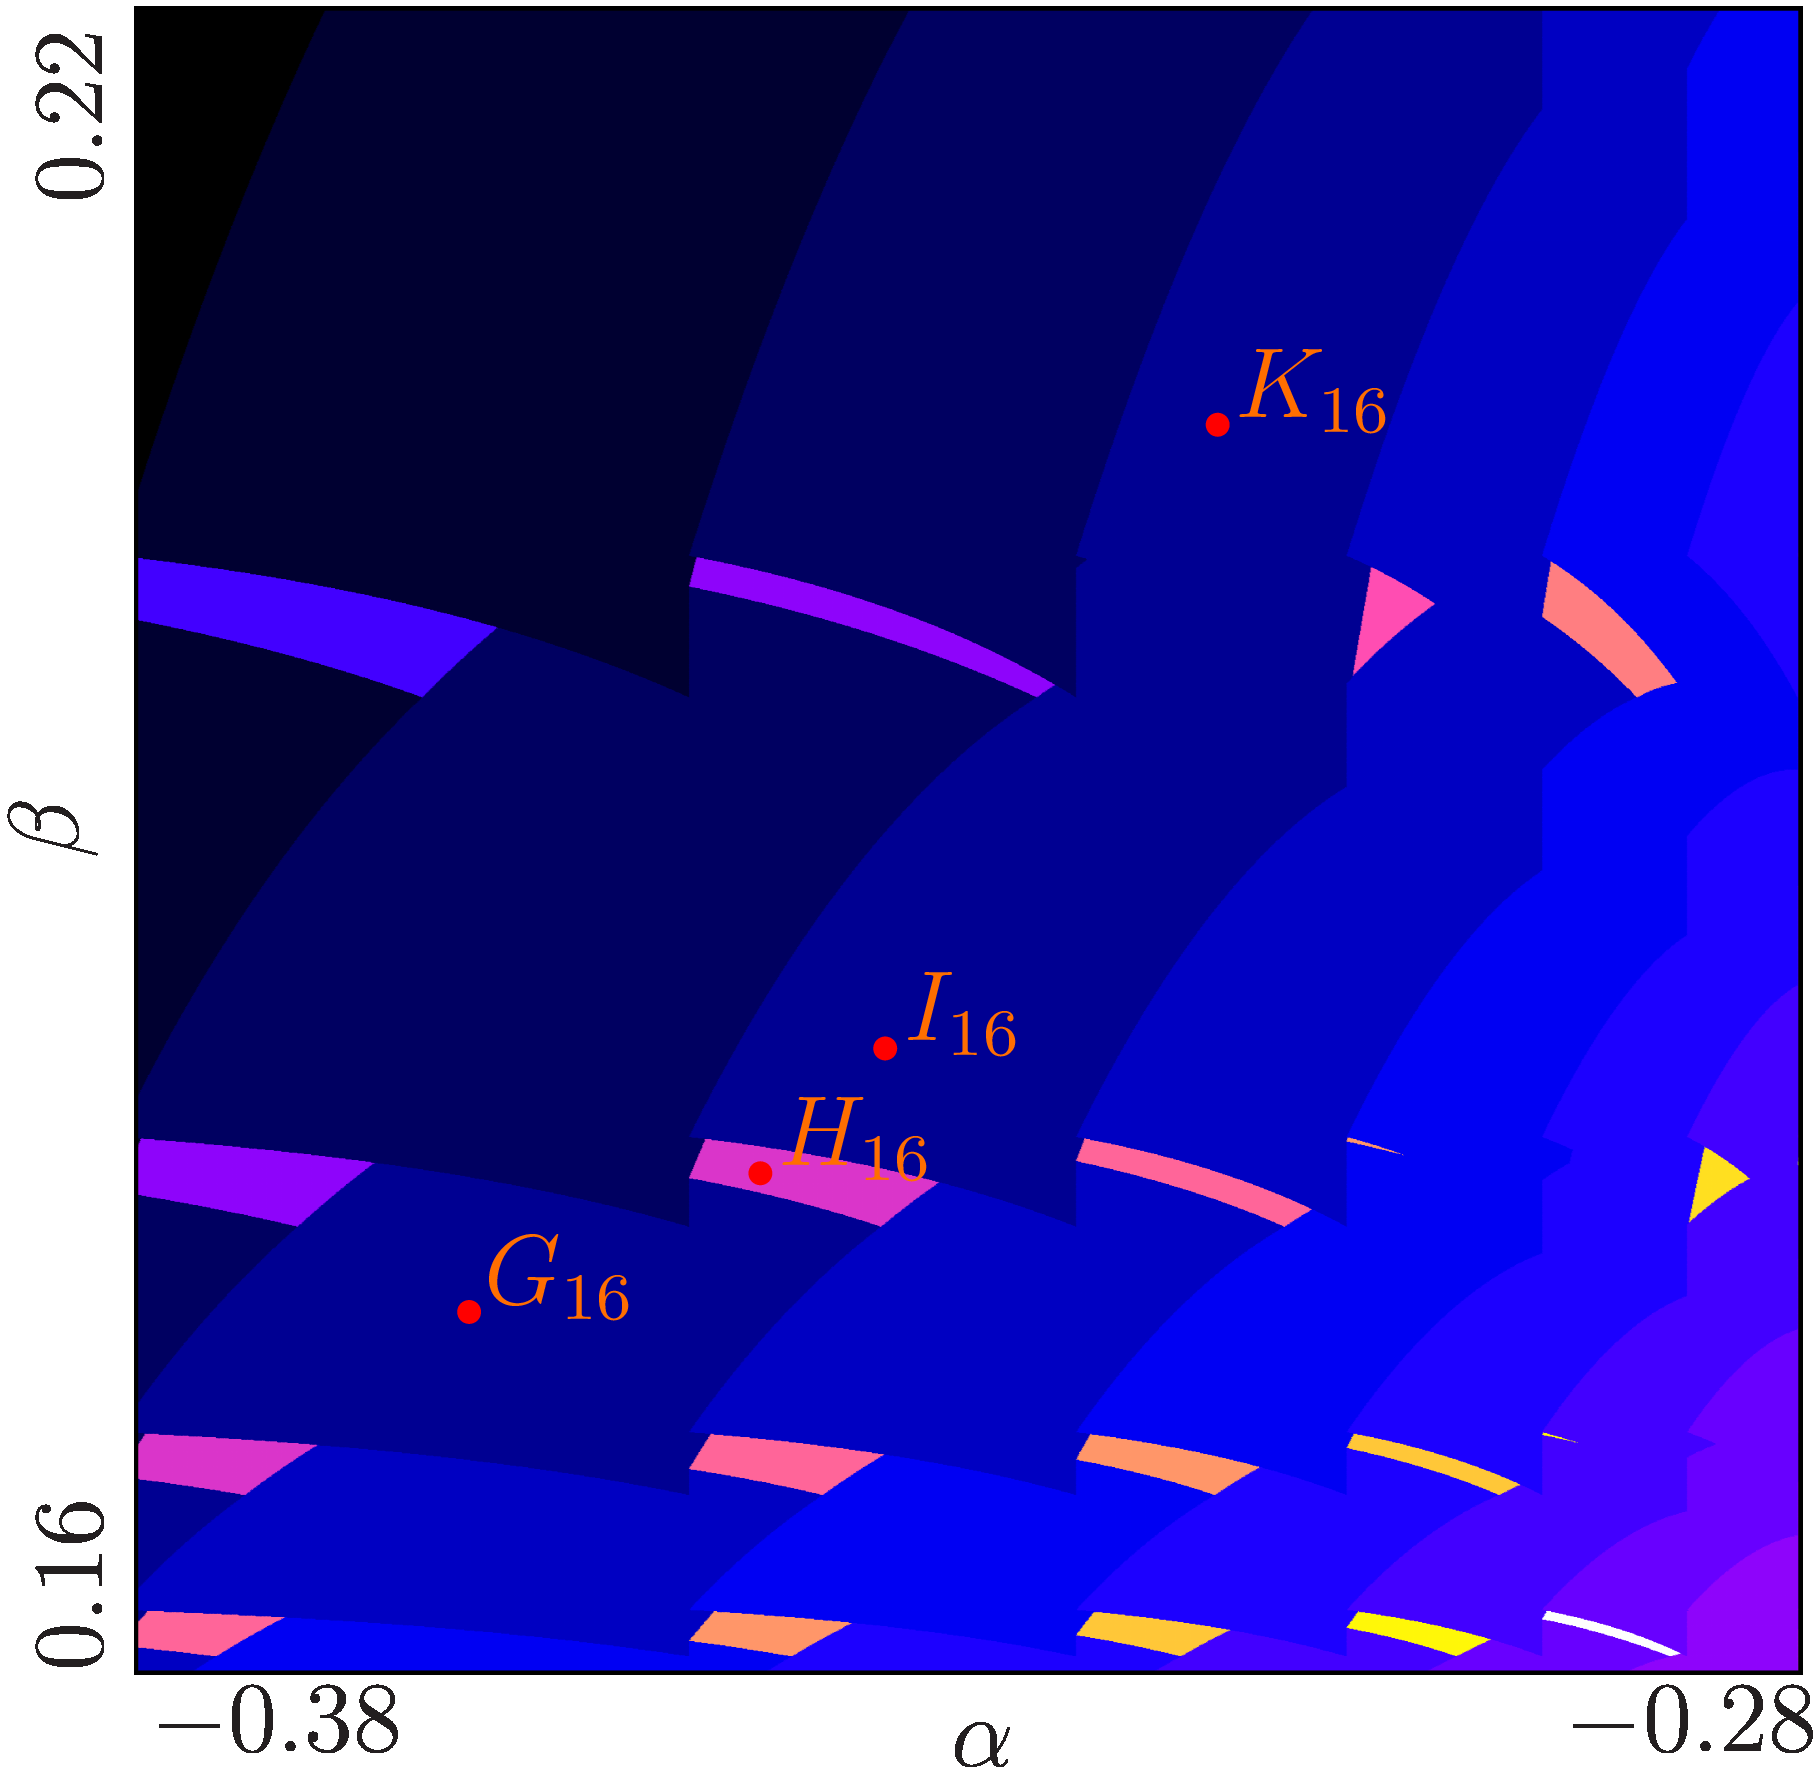
\includegraphics[width=.48 \textwidth]{../Figures/6/6.14a/result.png}
		\label{fig:arch.chainend.1}
	}
	\subfloat[Even larger values for $\beta$]{
		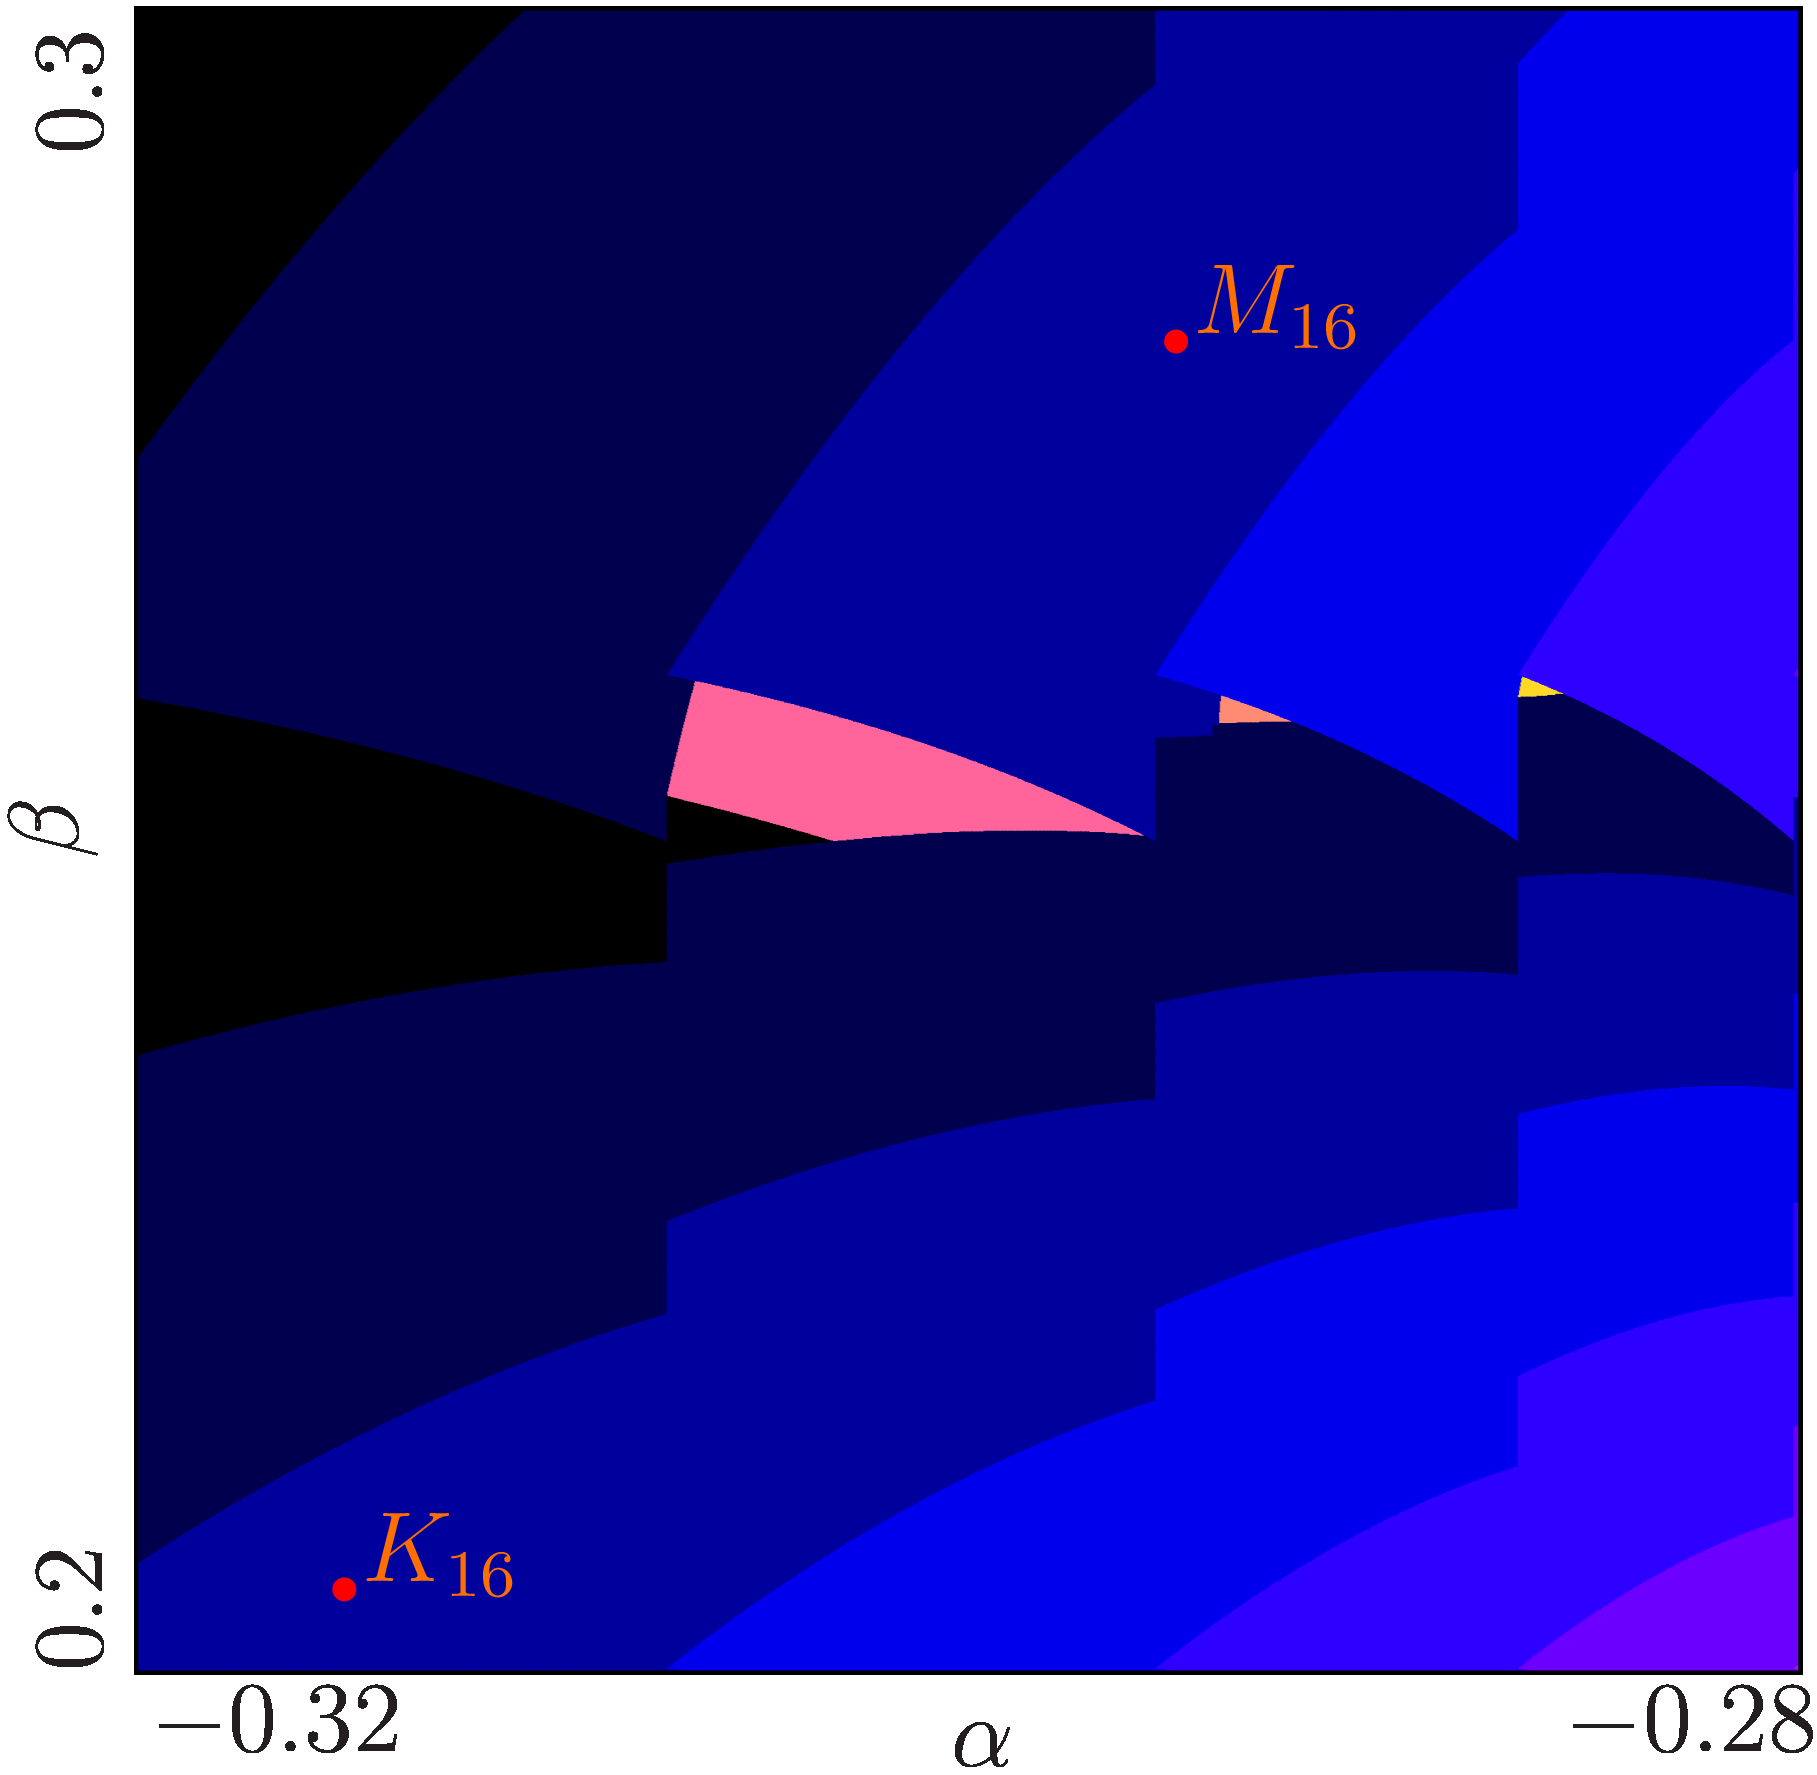
\includegraphics[width=.48 \textwidth]{../Figures/6/6.14b/result.png}
		\label{fig:arch.chainend.2}
	}
	\caption[2D scans of periods in the archetypal model showing the end of the chains]{
		2D scans of periods in the adjusted archetypal model showing the end of the chains of the same period.
		(a) shows the 2D scan for larger values of $\beta$ where ``type B'' regions start missing from the chain of period $16$.
		(b) shows the 2D scan for even larger values of $\beta$ where the chain is no longer connected.
	}
\end{figure}

\Cref{fig:arch.chainend.1} shows a 2D scan of the periods of the \hl{halved} archetypal model where the ``type B'' parameter regions in the chains are visible.
We can see that the ``type B'' parameter region \hl{in} \Cref{fig:arch.chainend.1} between the ``type A'' parameter region marked with point $I_{16}$ and the ``type A'' parameter region marked with point $K_{16}$ is missing.
There should have been the parameter region $\P_{\A^3\B^5\C^2\D^6, \A^2\B^6\C^3\B^5}$ according to the rules laid out in \Cref{sec:arch.dynamics}.

Furthermore, the chain is completely disconnected when looking at even higher values of $\beta$.
\Cref{fig:arch.chainend.2} shows this.
The parameter region $\P_{\A\B^7\C\D^7}$ marked with $M_{16}$ \hl{in} \Cref{fig:arch.chainend.2} is the predicted last ``type A'' parameter region of the chain with period $16$.
It is not connected to the second last parameter region $\P_{\A^2\B^6\C^2\D^6}$ marked with $K_{16}$ \hl{in} \Cref{fig:arch.chainend.2}.

This violates the rules and our expectation for the archetypal model.
\Citeauthor{akyuz2022} observed the same behavior in the original model in \cite{akyuz2022}.
He also looked at a chain of parameter regions with period $16$.
The chain behaved according to the rules up to the second last ``type A'' parameter region, $\P_{\A^2\B^6\C^2\D^6}$.
His hypothesis is that the scan of the periods done here is a two-dimensional one, while the model has more dimensions.
So choosing a different parameter plane for the 2D scan of the periods might reveal a perfect chain with period $16$~\cite{akyuz2022}.
This could also be the case here, since the archetypal model has $5$ parameters and the period scan is done in two dimensions also.
\hl{
	Two ways, one could perhaps obtain such complete chins are introduced next.
}

\hl{
	First, one could adjust the parameters $\alpha$ and $\beta$ to act differently for the values at the end of the chains.
	For example, the parameter $\beta$ influences the parameter $c_L$ directly in the archetypal model.
	But it could also influence some other parameters of the model when $\beta$ crosses some threshold.
	The same can be done for $\alpha$.
}

\hl{
	Secondly, one could try to force the model to behave in such a way, that the shape of the model function at some parameter values $\alpha_2$ and $\beta_2$ is the same as the shape of the model function at the parameter values $\alpha_1$ and $\beta_1$ shifted by $\frac{1}{4}$ where the parameter values $\alpha_1$ and $\beta_1$ belong to a parameter region at the start of a chain.
}
\hl{This can be expressed more precisely using} \Cref{equ:arch.dyn.shift}.
\begin{align}
	f_{\alpha_1, \beta_1}\left(x + \frac{1}{4}\right) & \equiv f_{\alpha_2, \beta_2}(x) \mod 1
	\label{equ:arch.dyn.shift}
\end{align}
\hl{
	This way, the stable cycle at the parameter values $\alpha_2$ and $\beta_2$ is $\Cycle{\A^{m-1}\B\C^{m-1}\D}$, provided the cycle at the beginning of the chain with parameter value $\alpha_1$ and $\beta_1$ is $\Cycle{\A\B^{m-1}\C\D^{m-1}}$.
	The newly chosen parameters should still act similar to the parameters $\alpha$ and $\beta$ in the archetypal model.
}
\hl{More specifically, the new parameter $\alpha$ needs to still have the same effect as in the archetypal model, but also the inverse effect of $\beta$ in the arcehtypal model to achieve the symmetry} \Cref{equ:arch.dyn.shift}.
\hl{
	The same is true for the new parameter $\beta$.
	Also, the model needs to have four quadratic branches.
}
\hl{This is therefore not possible with the archetypal model proposed in this thesis but can be achieved with the piecewise-quadratic model introduced in} \Cref{sec:setup.quad}.

